\documentclass[usenames,dvipsnames, 11pt]{beamer}

% \usepackage[latin1]{inputenc}
\usepackage{natbib}
\usepackage{amssymb}
\usepackage{amsmath}
\usepackage{minibox}
\usepackage{algorithmic}
\usepackage{algorithm}
\usepackage{graphicx,amsmath}

\usepackage{amsfonts}
\usepackage{amsthm}
% \usepackage[usenames,dvipsnames]{xcolor}
\usepackage{graphics}
\usepackage{subfigure}
\usepackage{setspace}
\usepackage{wrapfig}

% \usetheme{Boadilla}
% \usetheme{Berlin}
% \usetheme{Warsaw}
% \usetheme{AnnArbor}
% \usetheme{Antibes}
% \usetheme{CambridgeUS}
% \usetheme{Copenhagen}
% \usetheme{Darmstadt}
% \usetheme[height=5mm]{Singapore}
\usetheme{Amsterdam}
\usecolortheme{dolphin}
\usecolortheme[rgb={0,0.17,0.45}]{structure}

% \usetheme{EastLansing}

\setbeamertemplate{navigation symbols}{}
% \useoutertheme{infolines}

\addtolength{\textwidth}{6mm}

\def\newblock{\hskip .11em plus .33em minus .07em}

\newcommand{\aut}{\mathcal{A}_{\Sigma}}
\newcommand{\lang}[3]{\langle#1,#2,#3\rangle}
\newcommand{\makeimp}[2]{\textbf{\textcolor{#1}{#2}}}
\newtheorem{lem}{Lemma}
\newtheorem{thm}{Theorem}
\newcommand{\vek}[1]{{\bf {#1}}}
\newcommand{\vx}{{\vek{x}}}
\newcommand{\vy}{{\vek{y}}}
\newcommand{\vY}{{\vek{Y}}}
\newcommand{\vX}{{\vek{X}}}
\newcommand{\vv}{{\vek{v}}}
\newcommand{\vz}{{\vek{z}}}
\newcommand{\vtheta}{{\vek{\theta}}}
\newcommand{\vc}{{\vek{c}}}
\newcommand{\vw}{{\vek{w}}}
\newcommand{\vW}{{\vek{W}}}
\newcommand{\vf}{{\vek{f}}}
\newcommand{\vF}{{\vek{F}}}
\newcommand{\vwa}{{\vek{w}_{1\ldots r}}}
\newcommand{\vft}{{\vek{f}}}

\newcommand{\cV}{{\mbox{$\mathcal{V}$}}}
\newcommand{\cE}{{\mbox{$\mathcal{E}$}}}
\newcommand{\cY}{{\mbox{$\mathcal{Y}$}}}
\newcommand{\cX}{{\mbox{$\mathcal{X}$}}}
\newcommand{\cL}{{\mbox{$\mathcal{L}$}}}

\newcommand{\argmax}{{\text{argmax}}}
\newcommand{\argmin}{{\text{argmin}}}
\long\def\ignore#1{}
\long\def\todo#1{{{\bf TODO: } #1\\}}
\newcommand{\pd}[2]{\frac{\partial#1}{\partial#2}}

\newcommand{\indicate}[1]{[\![{#1}]\!]}
\newcommand{\acc}{{a}}
\newcommand{\vh}{{\vek{h}}}
\newcommand{\wt}{{p}}
\newcommand{\TP}{{A}}
\newcommand{\TPb}{{A}}
\newcommand{\estPerf}{{\hat{A}}}
\newcommand{\estURand}{{\hat{A}_R}}


\newcommand{\estSS}{{\mbox{$\hat{\mu}_S$}}}

\newcommand{\oracle}{{\mbox{Oracle}}}
\newcommand{\ham}{{\mbox{Ham}}}
\newcommand{\estSb}{{\mbox{$\hat{\mu}$}}}
%\newcommand{\estURand}{{\hat{A}_R}}
\newcommand{\sqErr}{{\mbox{Err}}}
\newcommand{\estSqErr}{{\mbox{EstErr}}}
\newcommand{\Err}{{\mbox{$\mathcal{E}$}}}
\newcommand{\loss}{{\mbox{$\mathcal{L}$}}}
\newcommand{\var}{{\sigma}}
\newcommand{\estVar}{{\mbox{$\hat{\sigma}$}}}
\newcommand{\nb}{{r}}
\newcommand{\feature}{{\vek{F}}}
\newcommand{\sign}{{\text{sign}}}
\newcommand{\cond}[1]{[\![{#1}]\!]^0_{-\infty}}

\newcommand{\Lp}{{L^1_k}} \newcommand{\Ln}{{L^2_k}}
\newcommand{\posf}{{f}}
\newcommand{\fp}{{{\posf_1}}} \newcommand{\fn}{{{\posf_2}}}
\newcommand{\np}{{{n_1}}} \newcommand{\nn}{{{n_{2}}}}
\newcommand{\minor}{{\text{minor}}}

\newlength{\wideitemsep}
\setlength{\wideitemsep}{\itemsep}
\addtolength{\wideitemsep}{1pt}
\let\olditem\item
\renewcommand{\item}{\setlength{\itemsep}{\wideitemsep}\olditem}


\title[{\makebox[.45\paperwidth]{Active Evaluation of Classifiers\hfill%
       \insertframenumber/\inserttotalframenumber}}]{Active Accuracy Estimation on Large Datasets}
\author {Namit Katariya, Arun Iyer, Sunita Sarawagi}
\institute{IIT Bombay}
% \date{}

\bibliographystyle{alpha}

\begin{document}
\begin{frame}
\titlepage
\begin{center}
\large{International Conference on Data Mining, 2012} \\ \vspace*{10pt}
\end{center}
\end{frame}

%%SS -- no need for an outline slide in a 15 min talk.
\AtBeginSection[]
{
  \begin{frame}{Outline}
    \tableofcontents[currentsection]
  \end{frame}
}

%%%%%%%%%%%%%%%%%%%%%%%%%%%%%%%%%%%%%%%%%%%%%%%%%%%%%%%%%%%%%%%%%%%%%%%%%%%%%%%

% Outline (number of slides in parantheses)
% 1. Goal (1)
% 2. Background
% i. Motivation (1)
% ii. Related work (1)
% iii. Our methods (1-2)
% 3. Results (4-5)
% 4. Summary (1)
% 5. Future work (1)
% 6. Backup slides (3-4)
\setbeamercovered{transparent}



\section{Problem setup}
\begin{frame}
\frametitle{Motivation}
\pause
\begin{itemize}
\item Setup
  \begin{itemize}
  \item A classifier $C(\vx)$ deployed on
  \item A large unlabeled dataset $D$
  \end{itemize}
  \pause
\item Estimate true accuracy $\mu$ of $C(\vx)$ on $D$
\pause
\item Given
  \begin{itemize}
\item A labeled set $L$ :  small or unrepresentative of $D$ 
\item \textcolor{blue}{Measured accuracy on labeled set $\neq$ True accuracy on data}
\item A human labeler
\end{itemize}
\end{itemize}
\end{frame}

%%SS do not make this a new section..put it in the same section as the first slide
% i do not know the beamer command for this.
% \section{Design goal}
\begin{frame}{Our goal}
\begin{enumerate}
%%SS -- format this better
\pause
\item \textcolor{Blue}{Handle arbitrary classifier} e.g. a user script
  \begin{itemize}
  \item existing work assumes that $C(\vx)$ is probabilistic and can output well-calibrated $\Pr(y|\vx)$ values.
  \end{itemize}
  \pause
\item \textcolor{Blue}{Provide interactive speed to user in loop even when $D$ is very large}
  \begin{itemize}
  \item even a full sequential scan on $D$ may not be practical. 
  \item $D$ can be accessed only via an index.
  \end{itemize}
  \pause
\item Require user to \textcolor{Blue}{label as few additional instances} as possible
  \begin{itemize}
  \item Similar to active learning but different ...
  %%SS -- copy reason from paper.
  \begin{itemize}
  \item Active learning usually used in the context of learning classifiers
  \item Task of learning classifier different from evaluating given classifier
  \end{itemize}
  \end{itemize}
  \end{enumerate}
\end{frame}

\begin{frame}{Outline}
The problem has two aspects \vspace{2mm}
\begin{enumerate}
\item \textbf{Accuracy estimation} (What this talk is about) \vspace{1mm}
\begin{itemize}
\item Given a fixed $L$ what is the best estimator of $\mu$? 
\item How to do this scalably on large $D$?
\end{itemize}
\vspace{3mm}
\item \textbf{Instance selection} (Not covered in this talk, details in paper)
\vspace{1mm}
\begin{itemize}
\item Selecting instances from $D$ to be labeled by a human and adding to $L$. Performed in a loop.
\end{itemize}
\end{enumerate}
\end{frame}

\section{Accuracy estimation}
\begin{frame}{Accuracy estimation}
\begin{itemize}
\pause
\item \emph{Simple averaged estimate} : $\hat{\mu}_R=\frac{1}{n}\sum_{i \in L}\acc_i$ is poor when $L$ is small or biased
\pause
\item A classical solution : \textcolor{Blue}{stratified estimate}
  \begin{itemize}
  \item Stratify $L$ and $D$ into $B$ buckets $(L_1,D_1),\ldots,(L_B,D_B)$ 
  \item Measure accuracy $\hat{\mu}_b$ of $L_b$ in each bucket $b$
  \item Estimate weight $w_b$ as fraction of instances in $D_b$
%%SS complete.
  \item Stratified estimate $\estSS=\sum_b{w_b\hat{\mu}_b}$
  \end{itemize}
  \pause
   \textcolor{Blue}{Error of $\estSS $ $<<$  Error of $\hat{\mu}_R$ if instances within a bucket are homogeneous}
\end{itemize}
\pause
Two challenges
\begin{enumerate}
\item Selecting a stratification strategy that \textcolor{Blue}{puts instances with same error in the same bucket}
\item \textcolor{Blue}{Finding $w_b$ scalably} when $D$ is large $\Rightarrow$ cannot stratify whole of $D$.
\end{enumerate}
\end{frame}

% \subsection{Stratification strategy}
\begin{frame}
\frametitle{Stratification strategy (h)}
\begin{itemize}
\pause
\item \textbf{Existing approach} : Bin $\Pr(y|\vx)$ values assumed to be provided by a classifier 
  \begin{itemize}
  \item \cite{bennett10} and \cite{druck11} %%SS (add the two citations).
  \item Not applicable since we wish to handle arbitrary classifiers.
  \end{itemize}
  \pause  
\item \textbf{Our Proposal} : 
  \begin{itemize}
  \pause
  \item $F(\vx,C):$ A feature represenation of the input $\vx$ and the result of deploying $C$ on  $\vx$
  \item Learn a hash function $h$ on features using the labeled data $L$
  \item \textcolor{Blue}{Stratification evolves as more labeled instances get added to $L$} (fixed in existing approaches)
  \end{itemize}
\end{itemize}
\end{frame}

%%SS --- Need to make it more detailed: state first about existing methods and why we needed to design a new one....Give an overview of our method and it key points.  what you have below is not good enough.
% \subsection{Learning hyperplanes}
\begin{frame}
\frametitle{Learning hyperplanes}
\pause
\begin{itemize}
\item \textbf{Existing methods} : Based on smoothing the objective and incrementally solving it
\pause
\begin{itemize}
\item \cite{norouzi2011minimal} penalizes large (small) hamming distance between similar (dissimilar) points. \textbf{Issue} : Bad local minimas. Poor results
\pause
\item \cite{kulis2009learning} specifies hash function in kernel form \& params are coefficients of these kernels. Solved using co-ordinate descent
\pause
\item \cite{wang2010sequential} proposes to sequentially update one hyperplane at a time. Also re-weight misclassified pairs of points while learning each subsequent hyperplane
\end{itemize}
\pause
\item \textbf{Our approach} : \textcolor{Blue}{Learn one hyperplane at a time}
\pause
\begin{itemize}
\item \emph{Relaxation} : Make use of the fact distance measure is over accuracy that usually takes 0/1 value
\item \emph{Optimization} : Allow groups formed by existing hyperplanes to choose their +ve \& -ve side after  optimizing for new hyperplane
\item \emph{Distinct hyperplanes} : Re-weight instances as in boosting
\end{itemize}
\end{itemize}
\end{frame}

%%SS -- give one slide technical summary.  what you had earlier was too high-level
% \subsection{Estimating bucket weights}
\begin{frame}
\frametitle{Estimating $w_b$ without sequentially hashing $D$}
\begin{itemize}
\pause
\item $\estSS=\sum_b{w_b\hat{\mu}_b}=\frac{1}{N}\sum_{i \in D}\hat{\mu}_{h(\vft_i)}$
\pause
\item Proposal sampling : $\hat{\mu}_{S_q} = \frac{1}{N}\left(\frac{1}{m}\sum_{i\in Q} \frac{\estSb_{h(\vft_i)}}{q(i)}\right)$
\pause
\item Optimal $q(i) \propto \estSb_{h(\vft_i)}$ : impossible without assigning each $i \in D$ to a bucket of $h(.)$
\pause
\item Allowed $q(i)$ are the ones which assign same probability to all instances $i$ within an index partition $D_u$ of $D$
\pause
\item \textbf{Claim} : Under above restriction, $q_u \propto \sqrt{\sum_{b}\estSb^2_b\wt(b|u)}$ where $\wt(b|u)$ is the fraction of  $i\in D_u$ with $h(\vft_i)=b$
\pause
\item $\wt(b|u)$ estimate : Initially depend on labeled data \& small static sample. Refine estimate as more instances get sampled from $D_u$
\pause
\end{itemize}
\end{frame}

%%%%%%%%%%%%%%%%%%%%%%%%%%%%%%%%%%%%%%%%%%%%%%%%%%%%%%%%%%%%%%%%%%%%%%%
\section{Results}
\begin{frame}
\frametitle{Results}

\only<1>{
\framesubtitle{Summary of datasets used}
\begin{itemize}
\item \textbf{TableAnnote} : Annotate columns of Web tables to type nodes of an ontology
\item \textbf{Spam} : Classifying web-pages as spam or not
\item \textbf{DNA} : Binary DNA classification task
\item \textbf{HomeGround, HomePredicted} : Dataset of (entity, web-page) instances and decide if web-page was a homepage for the entity
\end{itemize} \vspace{-5mm}
\begin{center}
\begin{table}
\centering
\begin{small}
\begin{tabular}{|l@{}|@{}r|@{}r|@{}r|@{}r|@{}r|}
\hline
Dataset & \multicolumn{1}{c}{\#} \vline & \multicolumn{2}{c}{Size} \vline & \multicolumn{2}{c}{Accuracy (\%)} \vline \\
 & \multicolumn{1}{c}{Features} \vline & \multicolumn{1}{c}{Seed($L$)} \vline & \multicolumn{1}{c}{Unlabeled($D$)} \vline & \multicolumn{1}{r}{Seed($L$)} \vline & \multicolumn{1}{r}{True($D$)} \vline \\
\hline
TableAnnote & 42 & 541 & 11,954,983 & 56.4 & 16.5 \\
Spam & 1000 & 5000 & 350,000 & 86.4 & 93.2 \\
DNA & 800 & 100,000 & 50,000,000 & 72.2 & 77.9 \\
HomeGround & 66 & 514 & 1060 & 50.4 & 32.8 \\
HomePredicted & 66 & 8658 & 13,951,053 & 83.2 & 93.9 \\
\hline
\end{tabular}
\end{small}
% \caption{Summary of Datasets}
\end{table}
\end{center}}

\only<2>{
\framesubtitle{Comparison of estimation strategies on the TableAnnote dataset}
\begin{center}
\begin{figure}
\includegraphics[width=0.75\hsize]{figs/e1axis.png}
\end{figure}
\small{
\begin{tabular}{|c l|}
\hline
\textcolor{MidnightBlue}{Random} & Random Sampling \\
\hline
\textcolor{Thistle}{PropSample} & Sampling from proposal distribution \\
\hline
\textcolor{OliveGreen}{ScoreBins} & Stratified sampling with scores \\
\hline
\end{tabular}}
\end{center}}

\only<3>{
\framesubtitle{Comparison of estimation strategies on remaining datasets}
\begin{center}
\begin{figure}
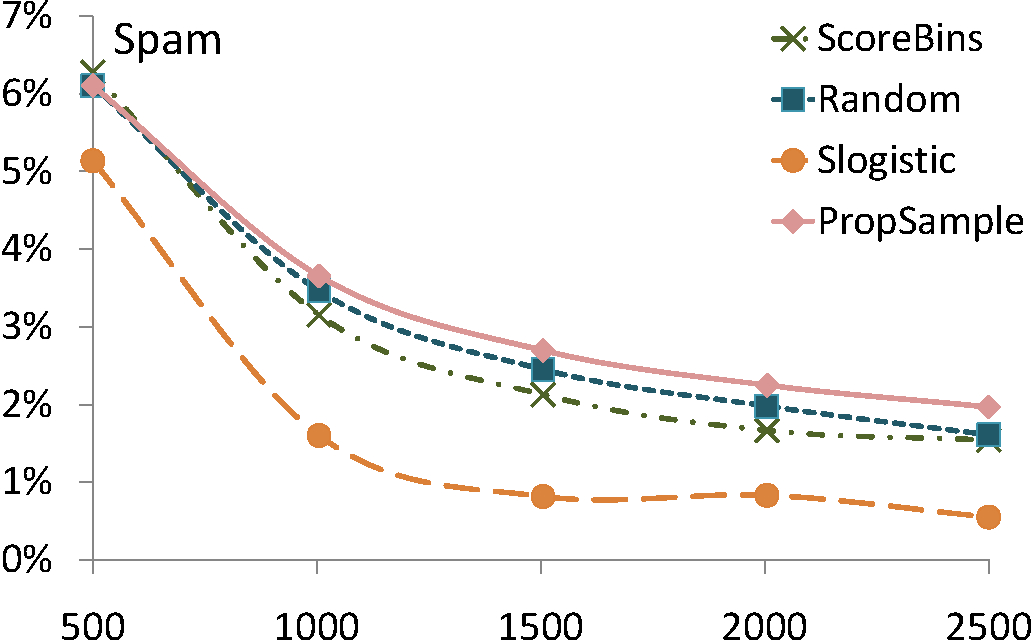
\includegraphics[width=0.37\hsize]{figs/e1spam_crop}
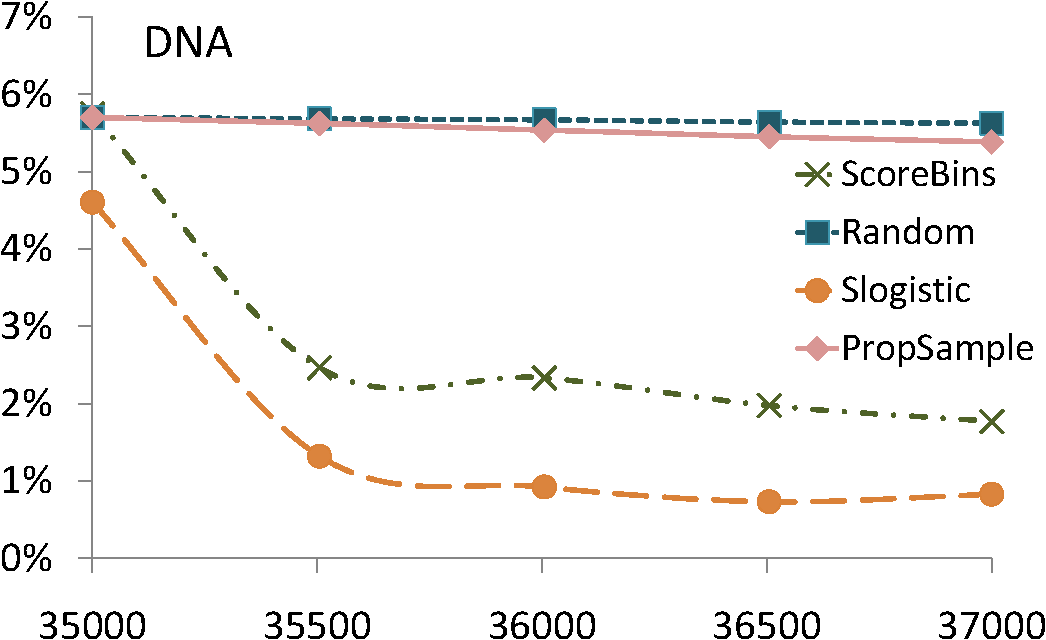
\includegraphics[width=0.37\hsize]{figs/e1dna_crop}
\end{figure}
\begin{figure}
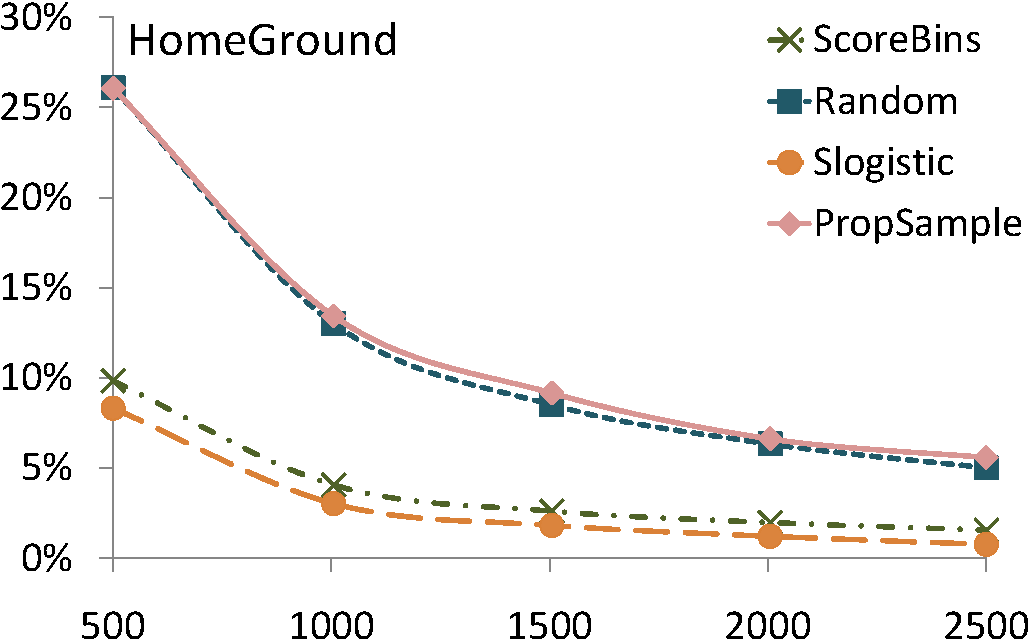
\includegraphics[width=0.37\hsize]{figs/e1homeground_crop}
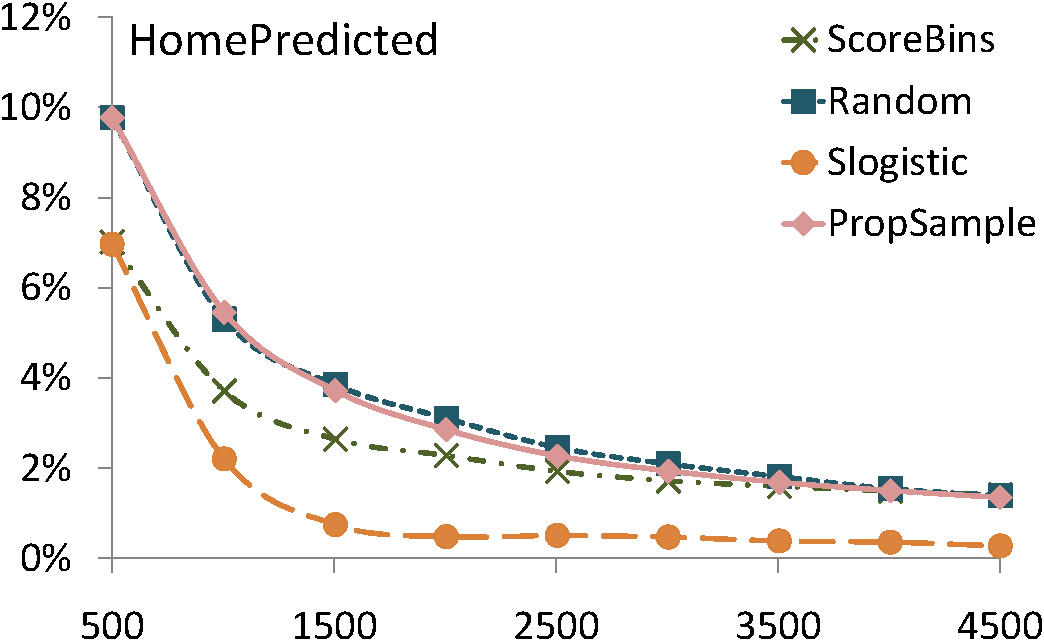
\includegraphics[width=0.37\hsize]{figs/e1homepredicted_crop}
\caption{Absolute error (on the $Y$ axis) of different estimation algorithms against increasing number of labeled instances (on the $X$ axis)}
\end{figure}
\end{center}}

\only<4>{
\framesubtitle{Comparison of different stratification methods on the TableAnnote dataset}
\begin{center}
\begin{figure}
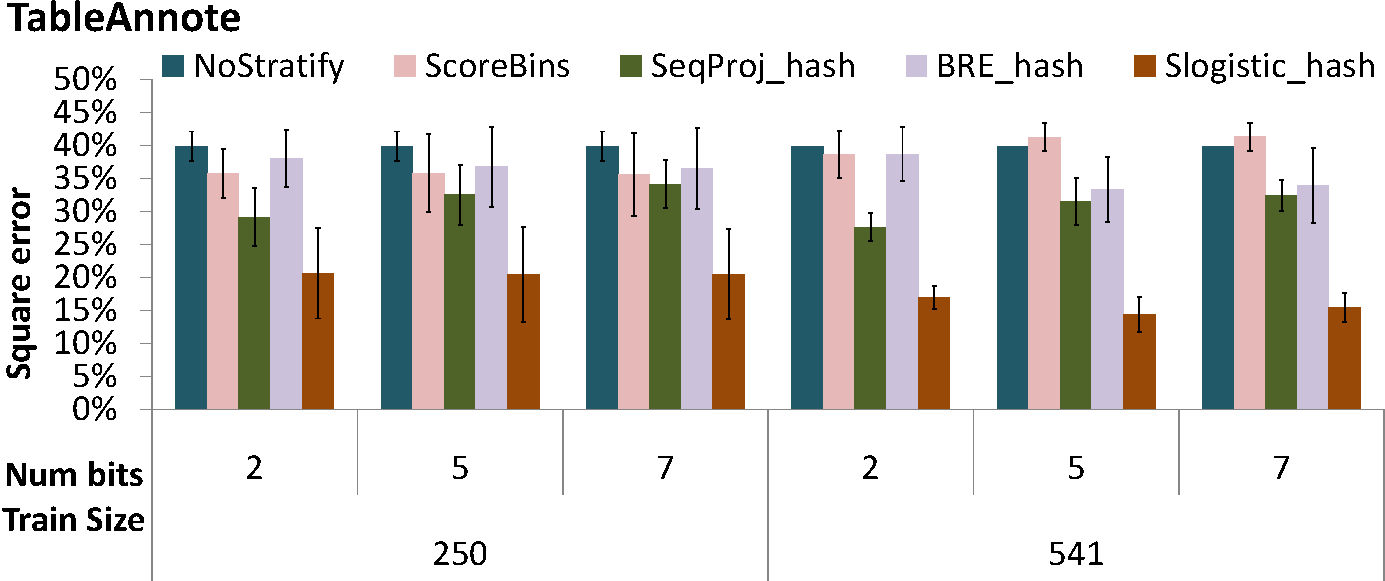
\includegraphics[width=\hsize]{figs/e2tableannote_crop}
%\caption{HomeGround data: Error of different stratification methods against increasing
% training sizes \& for different number of bits}
\end{figure}
\small{
\begin{tabular}{|c l|}
\hline
\textcolor{MidnightBlue}{NoStratify} & Simple averaging (no stratification) \\
\hline
\textcolor{Thistle}{ScoreBins} & Stratify using classifier scores \\
\hline
\textcolor{OliveGreen}{SeqProj\_hash} & Learn hyperplanes using method in \citep{wang2010sequential} \\
\hline
\textcolor{Orchid}{BRE\_hash} & Learn hyperplanes using method in \citep{kulis2009learning} \\
\hline
\end{tabular}}
\end{center}}

\only<5>{
\framesubtitle{Comparison of different stratification methods on remaining datasets}
\begin{center}
\begin{figure}
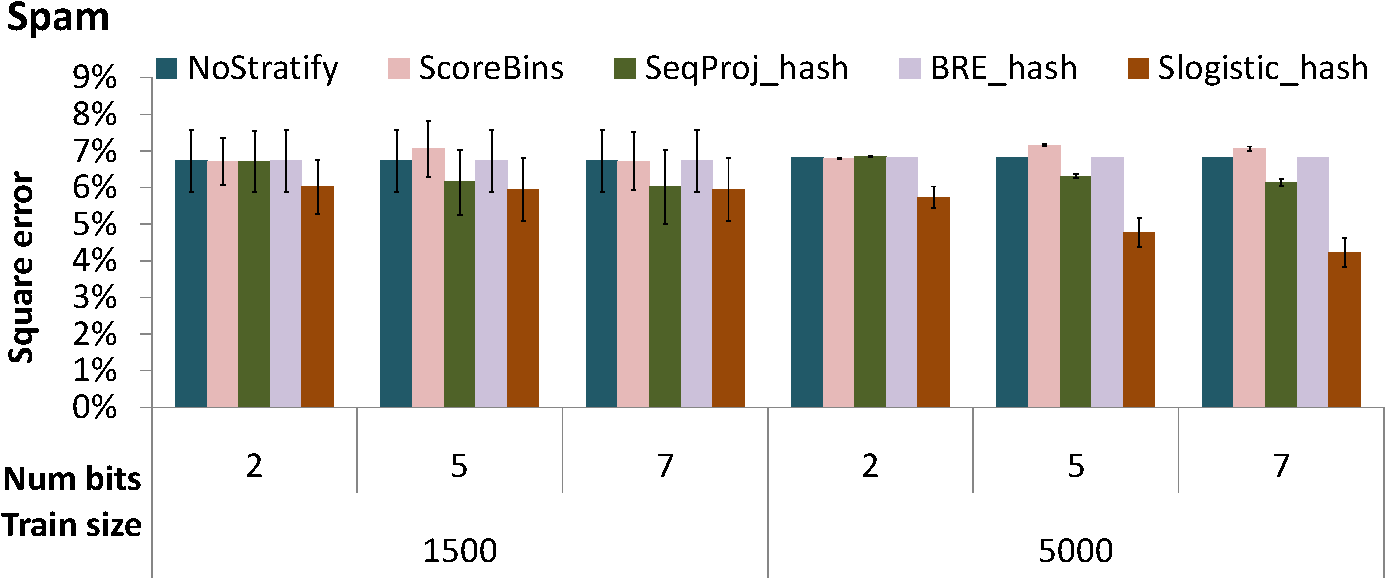
\includegraphics[width=0.5\hsize]{figs/e2spam_crop}
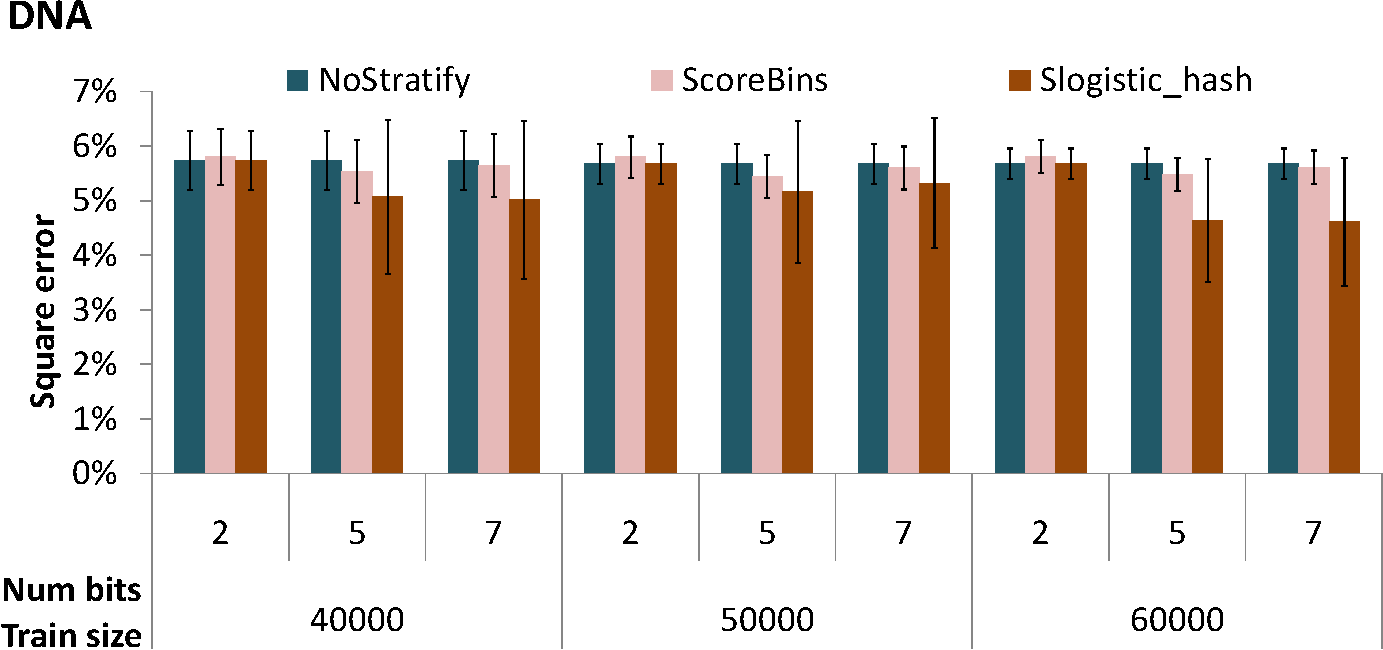
\includegraphics[width=0.5\hsize]{figs/e2dna_crop}
\end{figure}
\begin{figure}
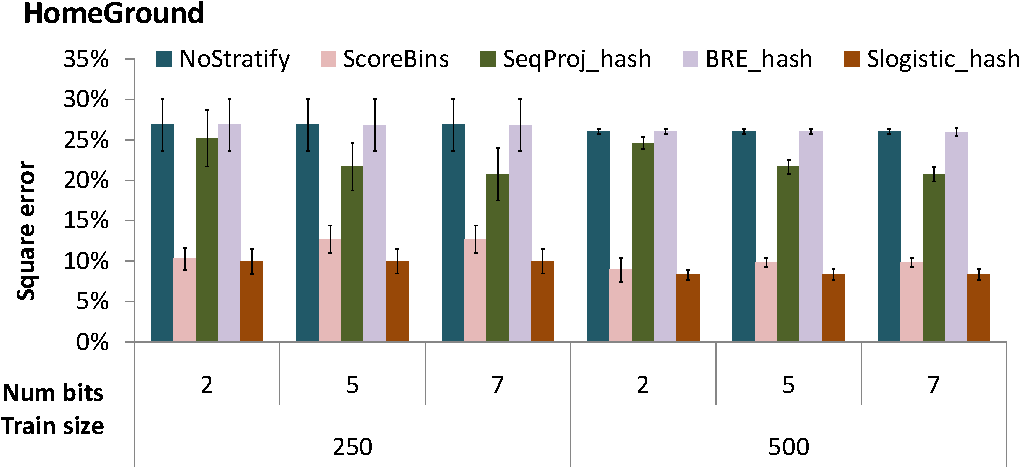
\includegraphics[width=0.5\hsize]{figs/e2homeground_crop}
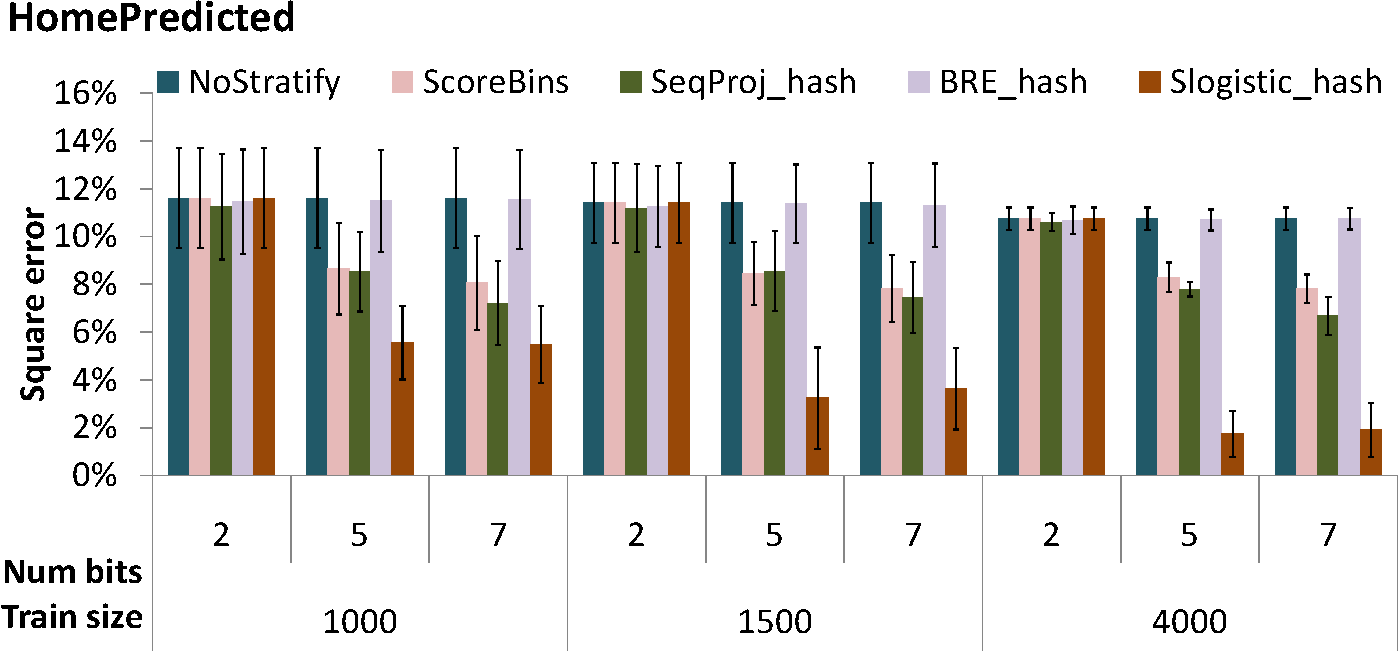
\includegraphics[width=0.5\hsize]{figs/e2homepredicted_crop}
\caption{Error of different stratification methods against increasing
  training sizes and for different number of bits}
\end{figure}
\end{center}}

\only<6>{
\framesubtitle{Comparison of methods of sampling from indexed data for estimating bucket weights}
\begin{figure}
\begin{center}
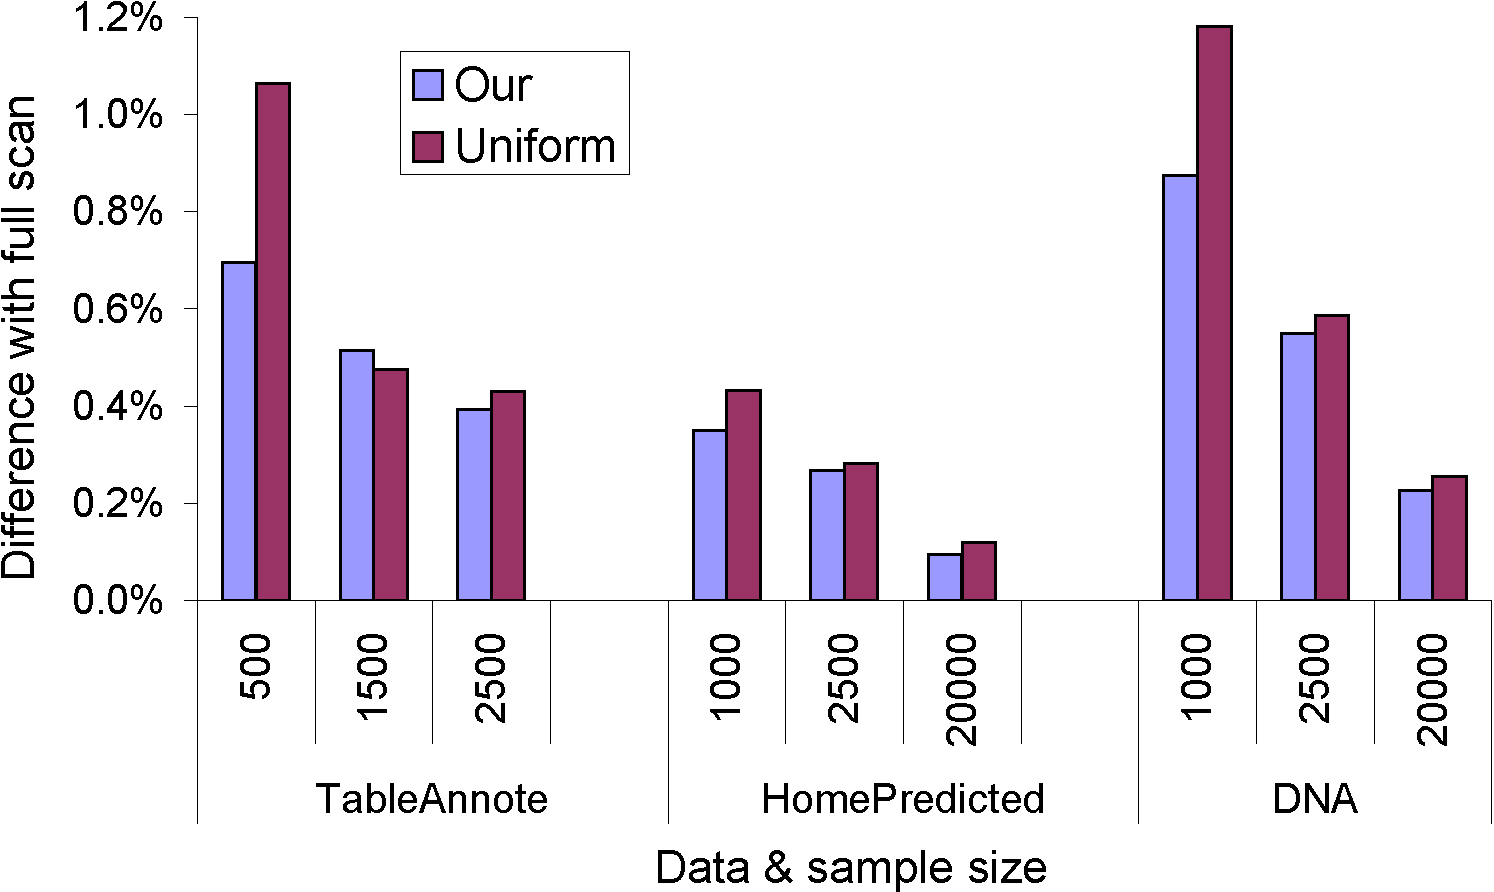
\includegraphics[width=0.85\hsize]{figs/allDataWts-crop}
\caption{Comparing methods of sampling from indexed data for
  estimating bucket weights}
\label{fig:allWts}
\end{center}
\end{figure}}

\end{frame}

%%%%%%%%%%%%%%%%%%%%%%%%%%%%%%%%%%%%%%%%%%%%%%%%%%%%%%%%%%%%%%%%%%%%%%

\section{Summary}
\begin{frame}{Summary}
\begin{enumerate}
\item Addressed the challenge of \emph{\textcolor{blue}{calibrating a classifier's accuracy on large unlabeled datasets} given small amounts of labeled data and a human labeler}
\pause
\item \textcolor{blue}{Proposed a stratified sampling-based method for accuracy estimation} that provides better estimates than simple averaging \& better selection of instances for labeling than random sampling
\pause
\item Between 15\% and 62\% relative reduction in error achieved compared to existing approaches
\pause
\item Algorithm made \emph{scalable} by proposing \textcolor{blue}{optimal sampling strategies for accessing indexed unlabeled data directly}
\pause
\item Close to optimal performance while reading three orders of magnitude fewer instances on large datasets
\end{enumerate}
\end{frame}

\begin{frame}
\frametitle{}
\begin{center}
\LARGE{Thank You}
\end{center}
\end{frame}

% \section{References}
\begin{frame}[allowframebreaks]{References}
\bibliography{report}
\end{frame}

%\begin{frame}
%\frametitle{Assigning Bucket Weights}
%\begin{itemize}
%\item Sample from a proposal distribution : $\hat{\mu}_{S_q} = \frac{1}{|S|}\sum\nolimits_{\vx\in S} \frac{1/N}{q(\vx)}\estSb_{h(\vx)}$
%\item \textbf{Result} : When $q(\vx)$ is restricted so that all instances within a partition $u$ are sampled with the same probability $q_u$,
%the expected squared error between $\hat{\mu}_{S_q}$ and $\estSS$ is minimized when
%\begin{center} $q_u \propto \sqrt{\sum_{b}\estSb^2_b\wt(b|u)}$ \end{center}
%\item $\wt(b|u)$ = fraction of instances in $D_u$ with $h(\vx)=b$
%\item Initially, use labeled data to estimate $\wt(b|u)$
%\item As more instances are sampled from any $D_u$, refine estimates of $\wt(b|u)$
%\end{itemize}
%\end{frame}
%
%\begin{frame}
%\frametitle{Instance Selection}
%\begin{itemize}
%\item Perform importance sampling where imp($\vx$) $\propto \estVar_{h(\vx)}$ without evaluating $h(\vx)$ over entire $D$
%\item Generate a larger sample $S$ via proposal distribution $q(\vx)$ restricted to choose same $q(\vx) ~\forall \vx$ in data
%partition $D_u$
%\item Then from $S$ generate the sample of $k$ instances by weighting each instance as $f(\vx)/q(\vx)$. Good only if $q(\vx) \sim f(\vx)$
%\item Best $q(\vx)$ found by solving for unlabeled bucket weights $q_1,\ldots,q_U$
%so that expected L1 distance between $f(\vx)$ and $q(\vx)$ is minimized
%\begin{center}
%$\min_{q_1,\ldots,q_U} \sum_u\sum_b \wt_u\wt(b|u) \left|\frac{\estVar_b}{Z_f} - q_u\right| ~s.t. \sum_u N\wt_uq_u=1$
%\end{center}
%\item $Z_f$ approximated as $\sum\nolimits_b\estVar_b\sum\nolimits_u\wt_u\wt(b|u)$
%\item Get $\wt(b|u)$ as explained in the previous slide
%\end{itemize}
%\end{frame}

\end{document}
